\chapter{Event Reconstruction in the CMS detector}
\label{chap:Event}

Events selected by the \ac{CMS} trigger system typically contain signatures of heavy particles, such as the top quark or the Higgs boson. However, the lifetime of these particles is extremely short and they travel a negligible distance before decaying into more stable particles, referred to as the final-state particles. Therefore, the reconstruction of an event produced in the proton-proton collisions requires the identification of all final state particles, which can be then used to infer the presence of heavy particles. Except for weakly interacting neutrinos, all final-state particles leave traces of their signatures in at least one subsystem of the \ac{CMS} detector as illustrated in Figure~\ref{fig:PF}.

\begin{figure}[tbh!]
 \begin{center}
 \begin{tabular}{c}
 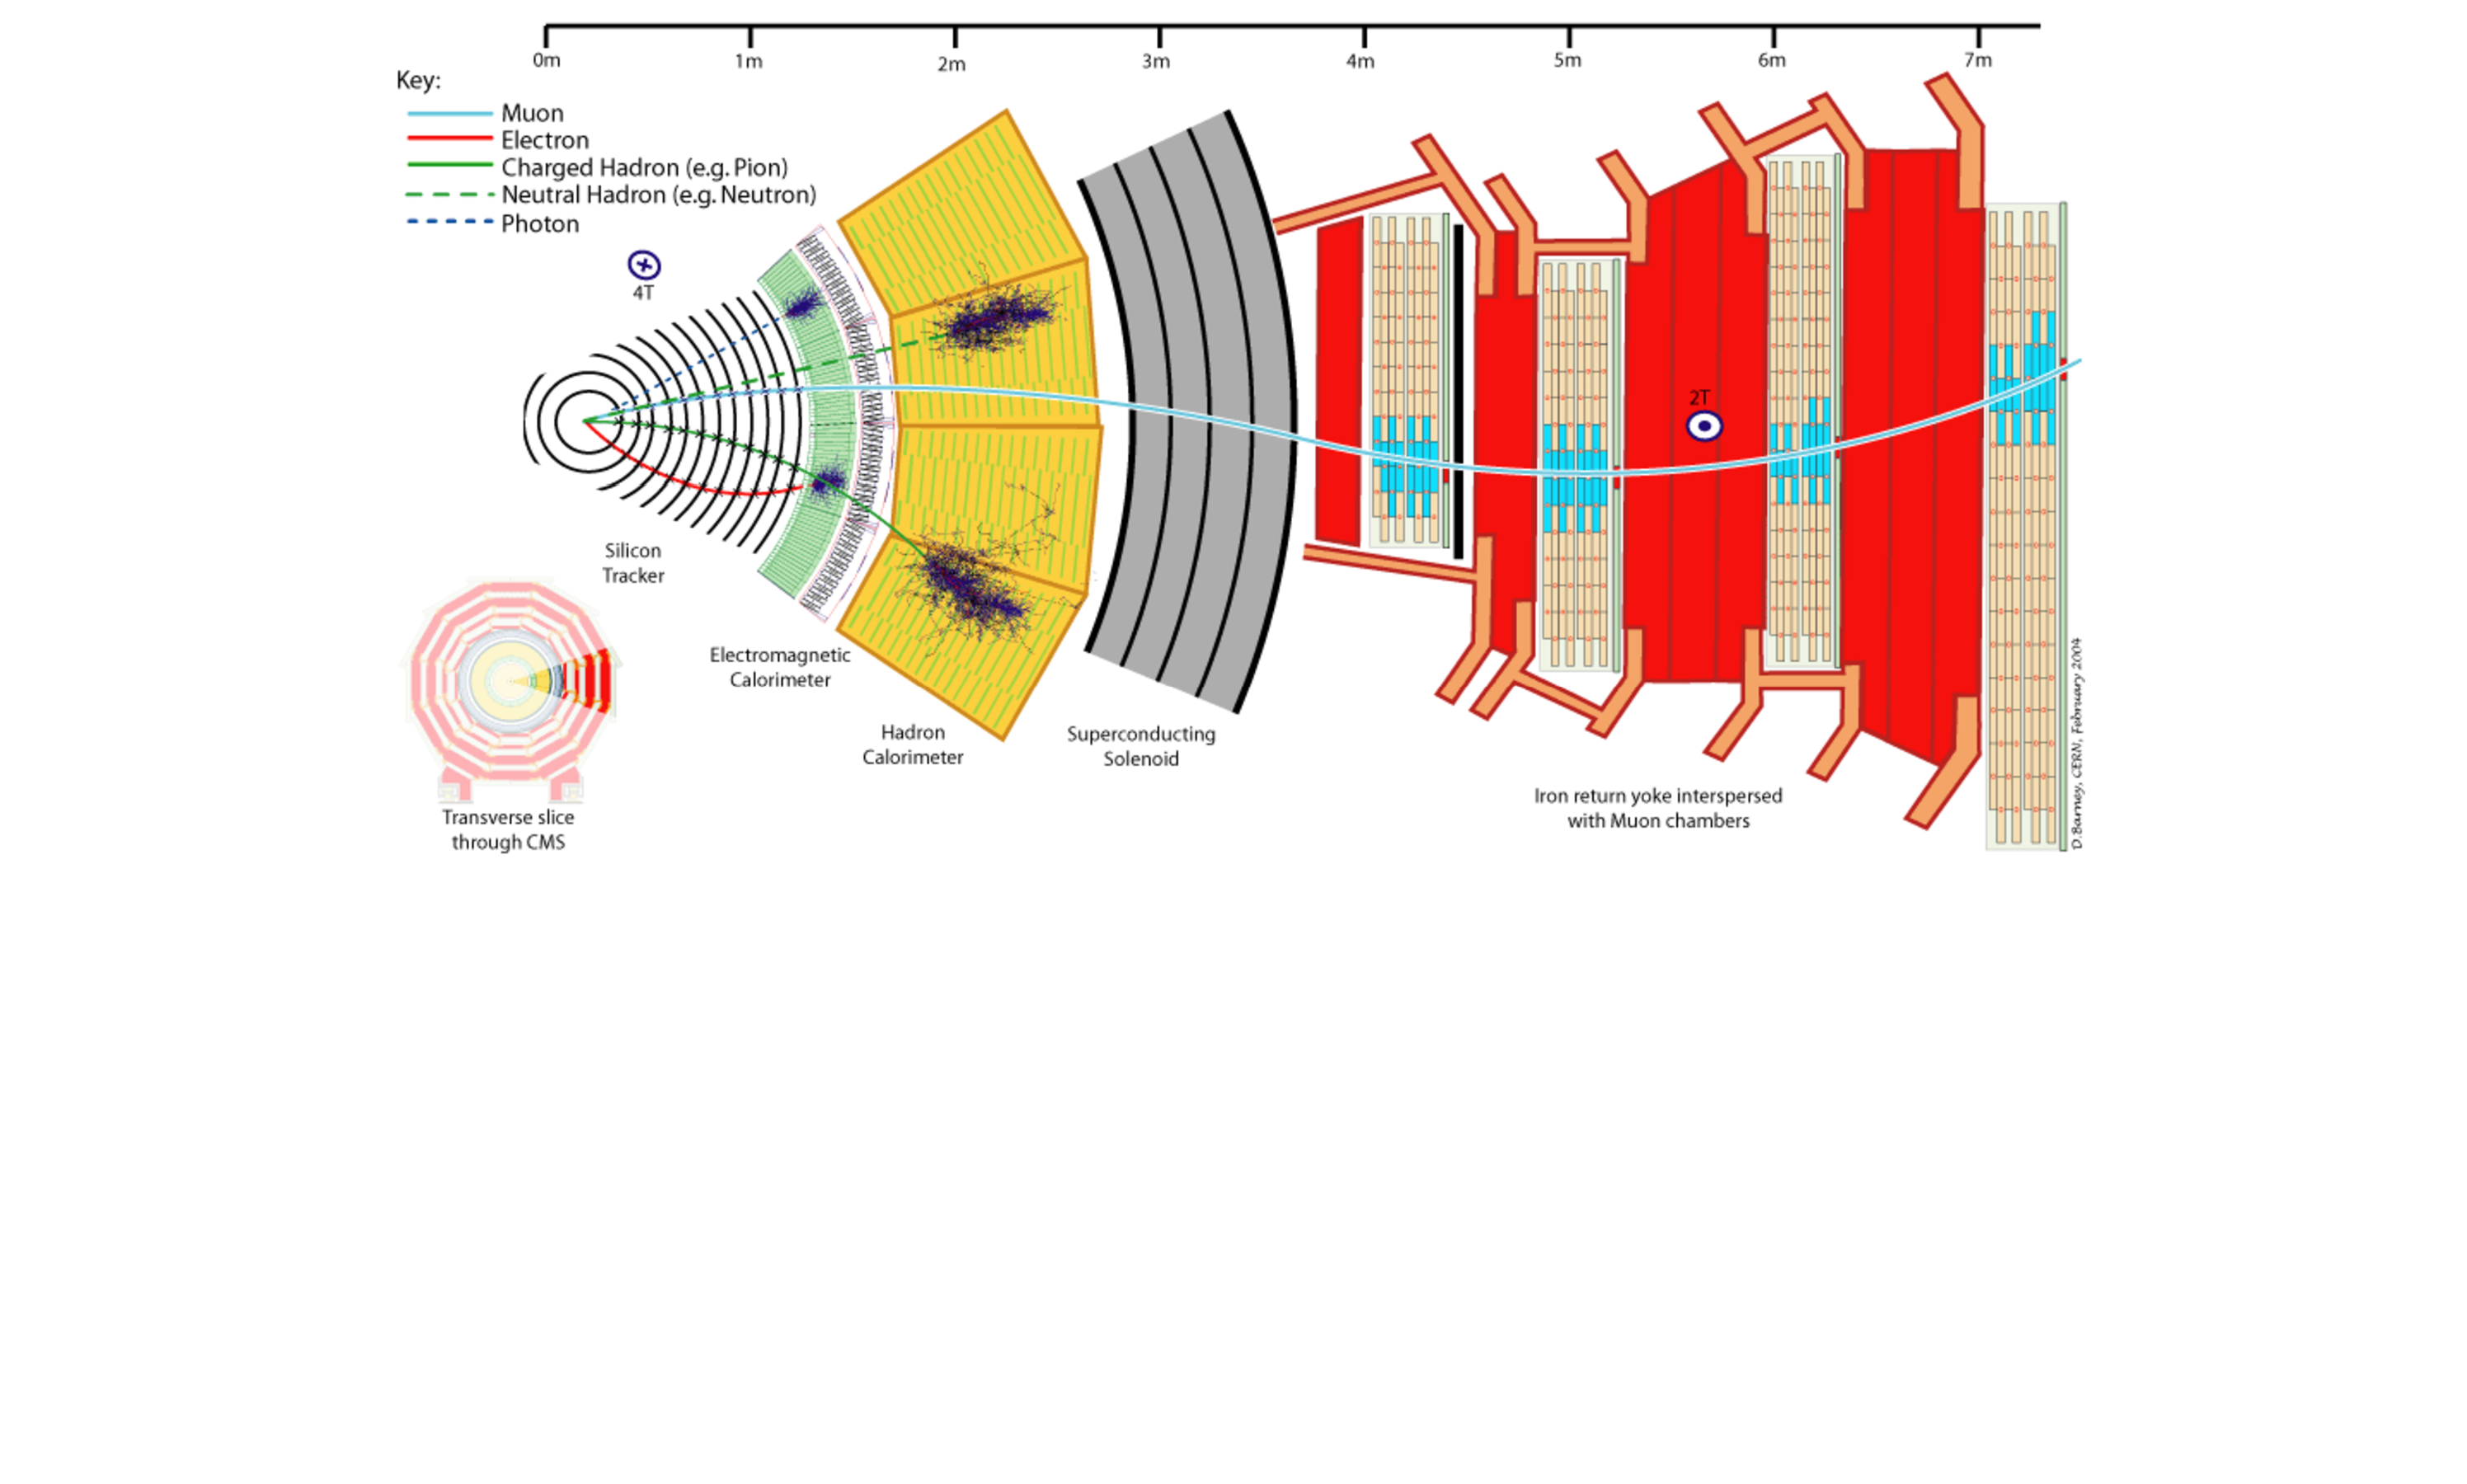
\includegraphics[width=0.9\textwidth]{figures/Part2/Event/PF}
 \end{tabular}
 \caption{A cross-sectional view of a slice of the \ac{CMS} detector in the transverse plane, adapted from~\cite{Barney:2018}. Paths of different particles that interact with various subsystems of the \ac{CMS} detector are highlighted.}
 \label{fig:PF}
 \end{center}
\end{figure}

The \ac{PF} algorithm~\cite{CMS:2017yfk} is used by the \ac{CMS} to combine measurements from all subsystems and provide a global event description. This algorithm consists of two main steps: i) reconstructing the \ac{PF} elements (i.e. tracks and calorimeter clusters) using information from various subsystems and ii) linking these \ac{PF} elements together to form the \ac{PF} candidates. The calorimeter clusters refer to a group of adjacent energy deposits in the calorimeters. The \ac{PF} candidates are labeled as electrons, photons, muons, charged hadrons, or neutral hadrons. Descriptions of the track and vertex reconstruction are given in \autoref{sec:Track}. The reconstruction of \ac{PF} electrons and muons are discussed in \autoref{sec:Electron} and \autoref{sec:Muon}, respectively. The \ac{PF} candidates are also used to reconstruct hadronic jets, taus, and \ac{MET}, which is discussed in \autoref{sec:Jet}, \autoref{sec:Tau}, and \autoref{sec:MET}, respectively.

\section{Track and Vertex}
\label{sec:Track}

Tracks from the inner tracking system and the muon system serve as one of the basic elements of the \ac{PF} algorithm. The standard track reconstruction algorithm at \ac{CMS} is the so-called \ac{CTF}~\cite{Speer:2005dp}, which is an extension of the \ac{KF} algorithm~\cite{Fruhwirth:1987fm} that combines the pattern recognition and parameter fitting. The procedure starts by forming a seed using only two or three hits. The initial estimate of the track parameters and their uncertainties are also made in the seeding stage. A \ac{KF}-based pattern recognition is then used to build track candidates by propagating the trajectory of each seed to its nearby surfaces. If a hit is found in the expected window it is added to the candidate track while the track parameter is updated at the same time. As illustrated in Figure~\ref{fig:CTF}, the improved knowledge of the track parameter as a result of newly added hits allows for a tighter window for the next propagation. 

\begin{figure}[tbh!]
 \begin{center}
 \begin{tabular}{c}
 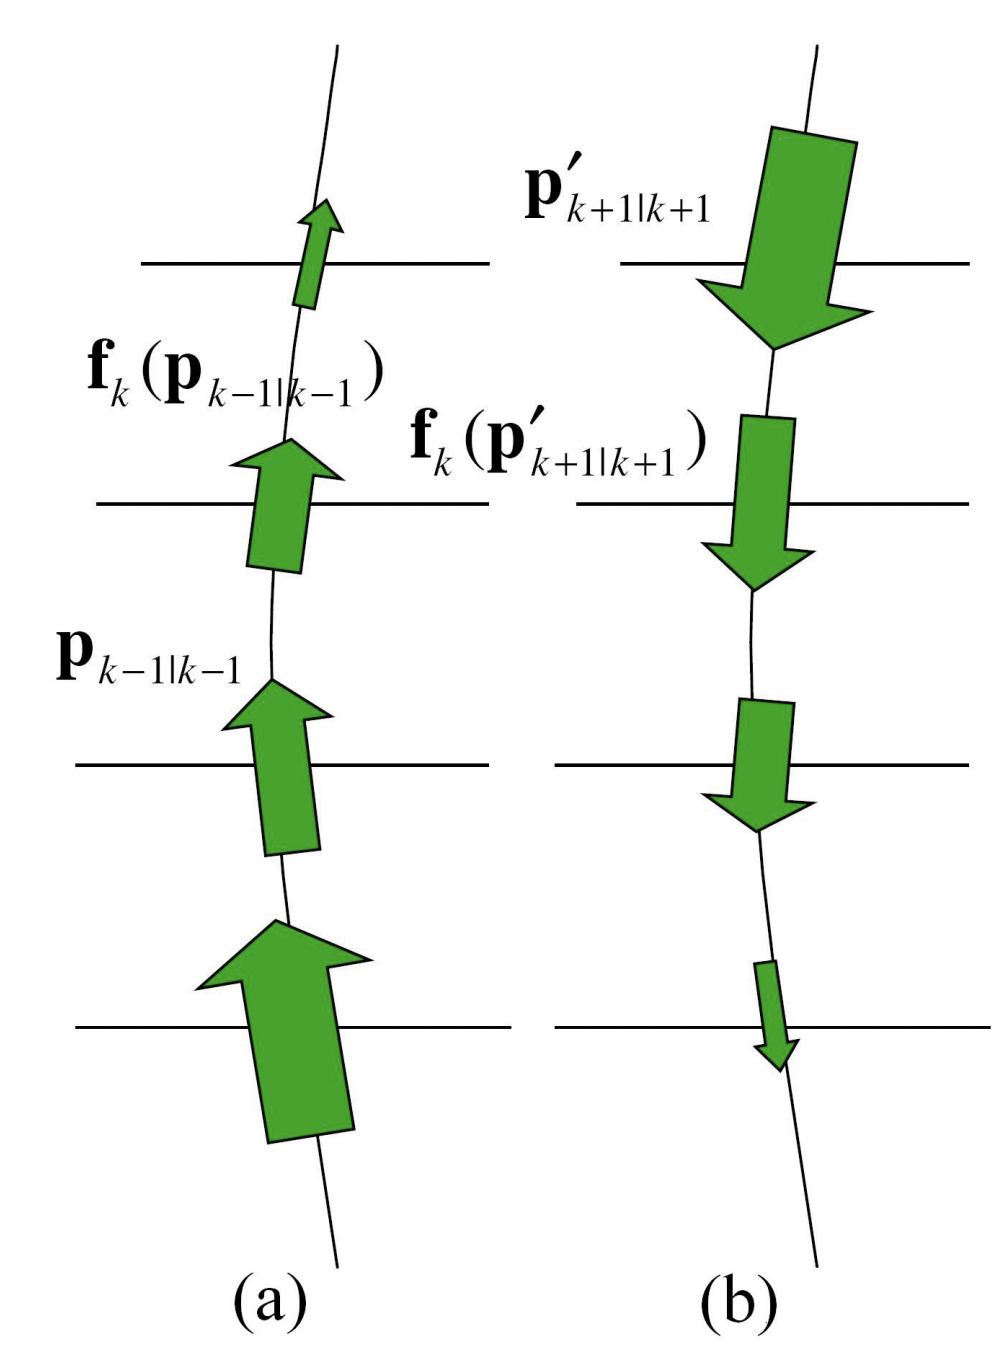
\includegraphics[width=0.4\textwidth]{figures/Part2/Event/CTF}
 \end{tabular}
 \caption{Illustration of the iterative tracking fitting in \ac{CTF}, adapted from~\cite{Lenzi:2008zza}. (a) shows the forward fitting while (b) shows the backward fitting. $\textbf{p}_{k-1|k-1}$ is the \ac{KF} state on surface $k-1$ calculated using the first $k-1$ hits. $\textbf{f}_{k}(\textbf{p}_{k-1|k-1})$ is the predicted \ac{KF} state on surface $k$. The size of the green arrows symbolizes the accuracy of the \ac{KF} state.}
 \label{fig:CTF}
 \end{center}
\end{figure}

The update of the track parameter is done using a \ac{KF} that performs an iterative fit to track parameters as new hits are added. Finally, a set of track quality selection criteria is applied to reduce the number of tracks that can not be associated with any particles, known as fake tracks. 

Reconstructed tracks can also be linked together to form a vertex. Vertices that are associated with inelastic scatterings of a collision event are known as the \ac{PV}. Due to the presence of \ac{PU}, multiple \acp{PV} exist in any given collision event. Three main steps are involved in the reconstruction of the \acp{PV}. Firstly, a set of selection criteria is applied to reconstructed tracks to ensure they are promptly produced in the collisions. Secondly, reconstructed tracks are clustered into a vertex candidate based on their $z$-coordinates using the deterministic annealing algorithm~\cite{Rose:1998dzq}. Finally, candidate vertices with more than one associated track are fitted using adaptive vertex fitter~\cite{Fruhwirth:2007hz}. For each event, the \ac{PV} with the highest $\sum\pt^2$ is often considered to be of the most importance to particle physicists as they carry the largest momentum transfer in an event. It is sometimes referred to as simply the \ac{PV} of an event while other \acp{PV} are considered to originate from \ac{PU}.

\section{Electron}
\label{sec:Electron}

Charged particles may emit photons in a process called the \emph{bremsstrahlung}. The intensity of this effect is inversely proportional to the squared mass of the charged particles. As the lightest charged particles, electrons produced in the hadron collisions are heavily affected by the bremsstrahlung effect, which comes in two different aspects. Firstly, the emission of a photon alters the electron trajectory, which undermines the performance of the standard tracking algorithm. A dedicated algorithm known as the \ac{GSF}~\cite{Adam_2005} is therefore used to fit the electron parameters. Moreover, the bremsstrahlung photons emitted by electrons often cause a more widespread pattern of \ac{ECAL} clusters along the $\phi$ direction. Therefore, multiple adjacent \ac{ECAL} clusters are combined to form the so-called \emph{superclusters}.

The electron reconstruction is fully integrated into the \ac{PF} framework, which associates \ac{GSF} tracks from the inner tracking system to the \ac{ECAL} clusters. The final assignment of the electron energy is based on a weighted combination of the \ac{ECAL} super cluster energy and tracker momentum~\cite{Baffioni:2006cd}. In addition to the electron reconstruction, identification criteria are often applied and optimized for different analyses. For both analyses described in this thesis, the primary objective of the electron identification is to control the contamination of the \emph{nonprompt} leptons. To this end, a \ac{BDT}-based electron identification is deployed, which is discussed in \autoref{sec:Leptons}.

\section{Muon}
\label{sec:Muon}

In \ac{CMS}, three types of muon tracks exist: standalone muons, tracker muons, and global muons~\cite{CMS:2018rym}. The standalone muons refer to the muon tracks reconstructed purely from hits in the muon system. The tracker muons are built ``inside-out'' by propagating tracks from the tracker to the muon system and matching it with at least one hit from either the \ac{CSC} or \ac{DT}. The global muon is reconstructed ``outside-in'' by: i) matching the standalone muons with the inner tracks and ii) performing a combined fit using the \ac{KF} to update the muon parameters. 

Same as the electron, the muon reconstruction is fully integrated into the \ac{PF} algorithm, which applies a set of selection criteria based on quality parameters in the muon reconstruction to the tracker muons and global muons. The so-called Medium muon ID~\cite{CMS:2018rym} is used by analyses described in this thesis. This ID accepts both tracker muons and global muons and adjusts the selection criteria accordingly. The overall efficiency of this ID is estimated to be around 99.5\% for muons from simulated W and Z events.

\section{Jet}
\label{sec:Jet}

The \ac{CMS} uses a sequential recombination algorithm, known as the anti-$k_t$ algorithm~\cite{Cacciari:2008gp}, to cluster \ac{PF} candidates into jets. The word ``$k_t$'' refers to the transverse momentum. This algorithm is designed to be \ac{IRC} safe, meaning the jet properties are invariant under the soft gluon emissions and collinear gluon splitting. The distance variable between two \ac{PF} candidates $i$ and $j$ in this algorithm is defined by 

\begin{equation}
\label{eq:ak}
d_{ij} = \min(\frac{1}{p_{\textsf{T}_i}^2},\frac{1}{p_{\textsf{T}_j}^2})\frac{\mathrm{\Delta}R_{ij}}{R},
\end{equation}

where $p_{\textsf{T}_i}$ and $p_{\textsf{T}_j}$ corresponds to the transverse momentum of \ac{PF} candidate $i$ and $j$ respectively. $\mathrm{\Delta}R_{ij}$ is the angular distance between the two objects defined by

\begin{equation}
\mathrm{\Delta}R_{ij} = \sqrt{\mathrm{\Delta}y_{ij}^2+\mathrm{\Delta}\phi_{ij}^2},
\label{eq:DDR}
\end{equation}

where $y=\frac{1}{2}\ln(\frac{E+p_z}{E-p_z})$, referred to as the rapidity, is not to be confused with the pseudorapidity $\eta$ defined in Equation~(\ref{eq:eta}). $R$ in Equation~(\ref{eq:DDR}) denotes the size of the jet which is typically chosen to be smaller than 1. For example, jets described later in this thesis are reconstructed with $R$ = 0.4. A second variable that measures the distance between particle $k$ and the beam axis in momentum space is defined as 

\begin{equation}
d_{kB} = \frac{1}{p_{\textsf{T}_k}^2}.
\end{equation}

The recombination procedure begins with calculating all combinations of $d_{ij}$ and concatenating them with every $d_{kB}$ to form the set $\{d_{ij}\}\cup\{d_{kB}\}$. The minimum of the entire set is then determined. If $d_{ij}$ is the minimum, then \ac{PF} candidates $i$ and $j$ are recombined into one candidate which replaces candidate $i$ and $j$ in the list. If $d_{kB}$ is the minimum, then it is labeled as a jet and removed from the list. This process is iterated until no \ac{PF} candidates are left. The name ``anti-$k_t$'' refers to the fact that the distance variable $d_{ij}$ is defined with respect to $k_t$ to the power of -2, which is different from the use of $k_t^2$ in $k_t$ algorithm~\cite{Ellis:1993tq}. 

As indicated in Equation~(\ref{eq:ak}), the anti-$k_t$ algorithm is dominated by hard particles. It typically starts with the hardest particle in an event and clusters and walks its way down to softer particles. The final momentum assignment of a jet is determined by the vectorial sum of the momenta of all particles that are clustered into this jet. The softest particles in an event are typically among the last ones to be clustered and they do not affect hard jets. The infrared safety is therefore guaranteed. Moreover, two collinear particles will also be given high priority to be merged because of the small $d_{ij}$ between them. This effectively ensures the collinear safety of the algorithm. Historically, sequential clustering algorithms are favored by theorists because of their \ac{IRC} properties but not favored by experimentalists due to their computational complexity. The introduction of the \textsc{FastJet} program~\cite{Cacciari:2011ma} improves significantly the the running speed of these sequential clustering algorithms, and they eventually become the standard jet clustering algorithm at the \ac{LHC}.

The measured energy of a jet is calibrated by applying a multiplicative factor $\mathcal{C}$ to each of its four-momentum components:

\begin{equation}
p^{\textsf{corr}}_{\mu} = \mathcal{C}\cdot p^{\textsf{raw}}_{\mu},
\end{equation}

where $\mathcal{C}$ is factorized into several components~\cite{CMS:2011shu},

\begin{equation}
\mathcal{C} = \mathcal{C}_{\textsf{offset}}(\pt^{\textsf{raw}})\cdot\mathcal{C}_{\textsf{MC}}(\pt^{\prime},\eta)\cdot\mathcal{C}_{\textsf{rel}}(\eta)\cdot\mathcal{C}_{\textsf{abs}}(\pt^{\prime\prime})
\end{equation}

where $\mathcal{C}_{\textsf{offset}}$ is the \ac{PU} offset correction that removes the energy coming from the \ac{PU} events. $\mathcal{C}_{\textsf{MC}}$ refers to the response correction. It accounts for the momentum difference between the reconstructed jets and particle-level jets. It is derived from simulation and applied to both data and \ac{MC}. The $\mathcal{C}_{\textsf{rel}}$ and $\mathcal{C}_{\textsf{abs}}$ correspond to the relative and absolute residual corrections, respectively. They account for the small differences in jet energy scale between data and \ac{MC} and are only applied to data.

\section{Hadronic Tau}
\label{sec:Tau}

Hadronic tau leptons are reconstructed with the \ac{HPS} algorithm~\cite{CMS:2011eio} in \ac{CMS}. This algorithm consists of several main steps: i) seeding, ii) ``strip'' reconstruction, iii) forming $\uptau_{h}$ candidates, and iv) choosing the final $\uptau_{h}$ object.

The \ac{HPS} algorithm uses \ac{PF} jets as ``seeds'' for the $\uptau_h$ candidates. It is required that \ac{PF} jets are reconstructed with the anti-$k_t$ algorithm with a distance parameter $R$ = 0.4. All \ac{PF} candidates within $\mathrm{\Delta}R~<$ 0.5 of the jets are considered in the following reconstruction steps.

Secondly, \ac{PF} electrons and photons in the seeding area are clustered into one or more rectangular windows (0.05$\times$0.2) in the $\eta-\phi$ plane known as ``strips''. Strips can be considered as proxies for the neutral hadron $\pi^0$, which appears in many decay modes of $\uptau_h$. Strips are narrow in $\eta$ direction but wider in $\phi$ direction to account for the bending of electrons by the magnetic field. $\uptau_h$ candidates typically have 0, 1, or 2 strips. 

Thirdly, charged hadrons with the highest energy (up to six) are combined with the strips to form $\uptau_h$ candidates. It is required that the combinations of strips and charged hadrons are compatible with one of the seven reconstructed decay modes listed in Table~\ref{tab:DM}.

\begin{table}[th]
\sffamily
\centering
\caption{Reconstructed decay modes of $\uptau_h$ expressed in combinations of reconstructed charged hadrons and strips and their targeted decay modes.}
\begin{tabular}{ccc}
\toprule
Reconstructed decay mode & DM & Targeted decay mode \\
\midrule
1 hadron & 0 & $\uptau_{h}^{\pm}\rightarrow h^{\pm}\nu_{\uptau} $\\
1 hadron + 1 strip & 1 & $\uptau_{h}^{\pm}\rightarrow h^{\pm}\pi^{0}\nu_{\uptau} $\\
1 hadron + 2 strips & 2 & $\uptau_{h}^{\pm}\rightarrow h^{\pm}\pi^{0}\pi^{0}\nu_{\uptau} $\\
2 hadrons + 0 strip & 5 & $\uptau_{h}^{\pm}\rightarrow h^{\pm}h^{\mp}h^{\pm}\nu_{\uptau} $\\
2 hadrons + 1 strip & 6 & $\uptau_{h}^{\pm}\rightarrow h^{\pm}h^{\mp}h^{\pm}\pi^{0}\nu_{\uptau} $\\
3 hadrons + 0 strip & 10 & $\uptau_{h}^{\pm}\rightarrow h^{\pm}h^{\mp}h^{\pm}\nu_{\uptau} $\\
3 hadron + 1 strip & 11 & $\uptau_{h}^{\pm}\rightarrow h^{\pm}h^{\mp}h^{\pm}\pi^{0}\nu_{\uptau} $\\
\bottomrule
\end{tabular}
\label{tab:DM}
\end{table}

``DM'' is a number assigned to each reconstructed decay mode, which is defined by 

\begin{equation}
\textsf{DM} = 5\times(N_{\textsf{prongs}}-1)+N_{\textsf{strips}}.
\end{equation}

DM = 5 or 6 corresponds to the scenario where one of the hadrons in a 3-prong $\uptau_h$ decay is not successfully reconstructed. The final assignment of a $\uptau_h$ candidate momentum is determined by the vectorial sum of all charged hadrons and strip constituents of that candidate. 

Finally, a set of selection criteria is applied to all $\uptau_h$ candidates. The candidate with the highest $\pt$ and passes all the selection criteria is chosen as the final $\uptau_h$ object. 

\section{Missing Transverse Momentum}
\label{sec:MET}

It is assumed that the initial transverse momentum in hadron collisions is zero. It is therefore very useful to compute the vectorial sum of momenta of all reconstructed objects in events to infer the presence of weakly interacting particles that escape detections, such as neutrinos or hypothetical dark matter particles. 

In \ac{CMS}, \ac{PF} candidates are used to reconstruct the \ac{MET} vector~\cite{CMS:2019ctu}:

\begin{equation}
\overrightarrow{p}_{\textsf{T}}^{\textsf{miss}} = -\sum_{i} \overrightarrow{p}_{\textsf{T}}^{i}.
\end{equation}

The magnitude of the \ac{MET} vector $\pt^{\textsf{miss}}$ is often considered to be analogous to $\pt$ of the particle that escapes the detector. 